\chapter{Utveckling av webbsida}
\label{sec: webb}

I utvecklingen av produkter i allmänhet är det viktigt att arbeta iterativt för att gradvis förbättra kvalitén på produkten. I utvecklingen av webbsidan har därför ett effektivt samarbete mellan produkt- och webbutveckling varit nödvändig. I detta avsnitt presenteras en kort bakgrund av produkt- och webbutveckling och därefter den övergripande metodik som genomsyrat arbetsprocessen. Slutligen redogörs för vad arbetsprocessen resulterat i och hur det har påverkat utvecklingen av webbsidans design och funktionalitet.  

\section{Bakgrund: produkt- och webbutveckling}
Genom att tidigt utgå från användarfeedback i ett utvecklingsarbete kan produkten bättre anpassas till användare, samt medföljande behov och krav. För ett sådant arbetssätt krävs en strukturerad metodik. Nedan beskrivs den övergripande processen för arbetssättet, samt några specifika metoder. Därefter beskrivs ett fåtal centrala begrepp i webbutveckling, samt de ramverk som används för att ta fram webbsidan i arbetet. 





\subsection{Produktutveckling - metodik, metoder och begrepp}
I ett produktutveckling behöver det initialt samlas in information om användaren och användningssituationen. I den initiala fasen används metoder som intervjuer, enkäter och observationer. Sedan krävs en analys av den insamlade informationen, för att få en djupare förståelse för användaren och situationen. Under analysen används statistiska metoder vid stora mängder kvantitativa data. Om informationen består av verbal data, från exempelvis öppna enkätfrågor eller intervjusvar, finns utarbetade metoder för att bearbeta informationen.
(uttryck på 25 procent mindre)


\emph{KJ-analys} är ett exempel på en sådan metod \cite{kj}. Därefter sker en fas av idégenerering. Med utgångspunkt från den insamlade och bearbetade informationen tas lösningar och koncept fram på de problem och behov som identifierats. Här finns metoder för att stimulera kreativitet. Exempelvis är \emph{Brainstorming} en specifik procedur för att generera ett stort antal idéer utifrån kreativt tänkande \cite{design}. Slutligen väljs ett koncept. Valet kan göras med hjälp av utarbetade metoder, men också utifrån utvecklarnas eget omdöme om vad som anses rimligt givet tid, resurser och kontext. 

\emph{KJ-analys}, eller släktskapsdiagram, är en metod för att strukturera stora mängder verbal information. Metoden kan användas för att gruppera användarbehov och krav i hierarkier, som sedan kan representeras i ett träddiagram. Resultatet är en grafisk bild av helheten, som samtidigt illustrerar samband mellan olika delar. Tillvägagångssättet är att successivt bygga upp en struktur genom att kategorisera de svar som mottagits. För varje enskilt svar, från exempelvis en öppen enkätfråga, ställs frågan om det svaret hör ihop med något av de tidigare svaren. Om ja, placeras svaret tillsammans i den identifierade kategorin. Om nej, får svaret utgöra en ny kategori. Vid repetition för samtliga svar kan de skapade kategorierna namnsättas och viktiga förhållanden kan sedan dras emellan dem. 

\emph{Intervju} är en frågebaserad metod för att få fram information ifrån användaren. För att få information av hög kvalité är det viktigt att typen av intervju, frågorna, och urvalet av intervjuobjekt tas i hänsyn. Det finns exempelvis \emph{strukturerade intervjuer}, \emph{semistrukturerade intervjuer}, och \emph{ostrukturerade intervjuer}. I en strukturerad intervju går utfrågaren igenom en på förhand utarbetad intervjumall. En semistrukturerad intervju utgår från en intervjumall, men utrymme ges för utvikningar på ämnen som kommer upp. Den semistrukturerade intervjun kategoriseras av fler följdfrågor för att få intervjuobjektet att utveckla sina svar. Ostrukturerade intervjuer utgår inte från en förbestämd intervjumall, utan är snarare ett öppet samtal kring ett förutbestämt ämne. 

%%Urvalet av deltagare kan ske utifrån olika urvalsprinciper till exempel statistisk representativt, teoretiskt representativt, teoretiskt kritiskt och bekvämlighetsurval. Statistiskt representativt urval är slumpvist utvalda deltagare av en tillräckligt stor mängd för att kunna få ett statistiskt signifikant resultat. Teoretisk representativt urval är medvetet utvalda deltagare, exempelvis från olika grupper av en större population. I ett teoretisk kritiskt urval utgår frågeställare från att det finns en viss grupp människor med speciellt hårda krav. Satisfieras gruppen har därmed hela gruppen tillfredsställts. Bekvämlighetsurval är ett urval av de deltagare som är lättast att få tag på.  

\emph{Brainstorming} är en metod som sker under en avsatt tid med syftet att utveckla en stor mängd idéer. Under tiden tas inte faktorer som användbarhet, realiserbarhet eller kostnad i hänsyn. Istället väntas kritiken till efter sessionen. Metoden bygger på deltagarnas kreativa potential, vilken ofta stimuleras av att se och höra andras idéer. Brainstorming sker oftast kring ett tema, exempelvis något som uppkommit från tidigare insamlad information. Utförandet kan se ut på många vis, men ett exempel är att låta deltagarna förbehållslöst skriva upp alla idéer de får på Post-It lappar eller en Whiteboard, och att idéerna därefter beskrivs och utvärderas.  

En minimalt funktionell produkt \emph{Minimum Viable Product} eller \emph{MVP} är en produkt med precis tillräckligt många funktioner för att tillfredställa tidiga användare och förse utvecklarna med information för vidare produktutveckling. En MVP är oftast ett mer tidseffektivt och billigare sätt att testa idéer och koncept än att bygga en produkt med mer komplett funktionalitet \cite{ries}. 

\subsection{Webbutveckling - grundläggande begrepp och ramverk}
Webbutveckling kan enkelt beskrivas som utvecklingen av applikationer, vars primära syfte är att visas och användas i en webbläsare. En webbapplikation kan förenklat sett delas upp i två delar: framsida och baksida. Framsidan är vad användaren ser och kan interagera med. Baksidan är logik på servar som användarna inte ser eller direkt kan interagera med, såsom databashantering, autentisering och svarsvalidering.

För att skapa framsidan används programmeringsspråken HTML, CSS och JavaScript. HTML står för Hypertext Markup Language, och utgör strukturen på det användaren ser. Exempelvis kontrolleras tabeller, inmatningsfält och rubriker genom detta statiska språk. CSS, eller Cascading Style Sheets används för att designa applikationen grafiskt. Med CSS kan element givna i HTML placeras ut eller animeras. JavaScript är ett programmeringspråk som kan användas för att dynamiskt flytta HTML-dokument eller kommunicera med baksidan genom HTTP-förfrågningar, ett protokoll för kommunikation mellan klienter och servrar. \cite{Webbutveckling}.

Med tiden har metoder för webbutveckling förbättrats och utvecklats, och sedan 2010 har ramverk som \emph{Vue}, \emph{Angular} och \emph{React} blivit populära \cite{webstats}. React används exempelvis för att förenkla, snabba upp, och möjliggöra skalbar utveckling av webbsidor. Förenklandet och skalbarheten uppnås bland annat genom en komponentbaserad modell som gör det lättare att återanvända och resonera kring delar av applikationen. Ökningen i hastighet sker genom användningen av en virtuell DOM (eng. \emph{Document Object Model}).

En DOM är ett API, eller applikationsprogrammeringsgränssnitt, som definierar logiken bakom strukturen i HTML och XML-dokument (där XML är ett annan Markup Language). Modellen ger en lättnavigerad och lättbygd struktur i dokumenten. I webbutveckling visualiseras HTML med hjälp av en DOM, men i React implementeras en ytterligare virtuell DOM mellan hemsidan och HTML-koden. Detta låter komponenter uppdateras snabbare och möjliggör ett dynamiskt användargränssnitt, utan att användaren märker det.

%%\subsection{Relationsdatabas}
En relationsdatabas är en samling datapunkter, vars värden kopplas via förbestämda relationer, som sedan kan kommas åt med hjälp av nycklar. Dessa nycklar måste vara unika, vilket kan exemplifieras i verklighetsexemplet i hur ett personnummer enbart måste kunna knytas till en unik person. SQL är ett av många exempel på språk som används för att komma åt den mängd data i databasen.  (koppla detta styckte till att datan behövs i djupinlärningen!)

Att implementera en koppling mellan databasen, och utföra operationer på datan som hämtas därifrån är nödvändigt för att kunna bygga stora applikationer utan att försämra prestanda eller skriva överkomplicerad kod. De olika lager (tidigare nämnda som framsida och baksida) är då 'abstraktionslager' för varje enskild del.

%%\subsection{GraphQL och Apollo}
\emph{Apollo} är en vanlig klient för att hantera GraphQL. Ett vanligt sätt att implementera en koppling till databasen är via ett REST-api. REST, som står för representational state transfer, är ett begrepp som beskriver ett sätt att hantera transaktioner mellan maskiner.

En nackdel med REST-api är att det ofta bygger på en enhetlighet, vilket skapar beroende, och långsamma utvecklingsmiljöer mellan lager inom framsida och baksida. Enkelt förklarat behöver utvecklare ofta i förväg definiera hur en applikation är tänkt att användas, och behöver därför lägga till så kallade 'endpoints' för nya användarfall.

\section{Metod}
Nedan följer metodiken bakom utvecklandet av webbsidan. Först beskrivs det översiktliga sambandet mellan parterna, varefter arbetet beskrivs på detaljnivå.

\subsection{Begränsningar och Förhållningspunkter}
Projektets utformning skapar utmaningen att på snabbast möjliga tid skapa en fullt fungerande och skalbar hemsida. webbsidan måste vara fullt fungerande av två skäl. För det första måste webbsidan användas i en riktig situation för att få verklig data på studenternas studiemönster för att kunna ge korrekta förutsägelser. För det andra behöver webbsidan vara fullt fungerande för att undvika att utveckla funktionalitet som inte fungerar i en verklig användningssituation. Webbsidan måste också vara skalbar, dvs det ska gå att öka antalet kurser och användare på sidan utan att skapa problem. Tidskravet är viktigt eftersom projektet förhåller sig till de tidsgränser som de faktiska kurserna sätter, såsom kursstart och tentavecka. 

\subsection{Iterationsprocess}

För att optimera samarbetet mellan produkt- och webbutvecklingen krävdes ett strukturerat informationsflöde samt tydliga processer. Produktutvecklingens ansvar var att samla in information om webbsidan och användningen och sedan analysera informationen för att ta fram koncept, designförslag och förbättringspunkter. Webbutvecklingens ansvar var att implementera design och förbättringspunkter, förse studenterna med en stabil och funktionell webbsida samt generera användarstatistik till produktutvecklingen.  
Visualiseringsprogrammet \emph{Figma} användes för att grafisk designa koncept på gränssnittet. Webbutvecklarna använde därefter filer från Figma för att utveckla applikationen. En anslagstavla etablerades i task-managerprogrammet \emph{Trello}, där produktutvecklaren kunde distribuera mindre arbetsmoment och förbättringspunkter att implementeras av webbutvecklarna. Efter att en ny funktion eller förbättringspunkt implementerats kunde produktutvecklaren följa upp detta med intervjuer med användarna eller användarstatistik från webbsidan.   

vi vi vi 

utgå ifrån bilden

\begin{center}
\begin{figure}[H]
    \centering
    \resizebox {0.7\textwidth} {!} {
        \definecolor{klight_green_400}{RGB}{156, 204, 101}

\tikzset{%
  project part/.style={
    rectangle,
    draw,
    fill=klight_green_400,
    thick,
    minimum width=3.2cm,
    minimum height=1.2cm
  },
  main line/.style={
    draw,
    line width=1mm,
    opacity=1,
    minimum size=1cm
  },
}

\begin{tikzpicture}[x=1.5cm, y=1.5cm, ->,>=stealth',auto, thick, line width=0.5mm, every node/.style={scale=1.3}]
% Base project nodes
\node [project part/.try] (collect) at (2,2) {$\textbf{Information}$};
\node [project part/.try] (concept) at (0,0) {$\textbf{Koncept}$};
\node [project part/.try] (use) at (4,0) {$\textbf{Användning}$};
\node [project part/.try] (implement) at (2,-2) {$\textbf{Implementation}$};


% Connect them 
\path[main line/.style={font=\sffamily\small}]
    (collect) edge[bend right] node[align=center, xshift=-1mm] [left] {\large KJ-analys, \\ \large idégenerering} (concept)
    (concept) edge[bend right] node [left] {\large Figma} (implement)
    (implement) edge[bend right] node[align=center, xshift=1mm] [right] {\large React, \\ \large GraphQL} (use)
    (use) edge[bend right] node[align=center, xshift=1mm] [right] {\large Intervjuer, \\ \large statistik} (collect);
\end{tikzpicture}
    }
    \caption{Iterationsprocess produkt-  och webbutveckling. Figuren visar de huvudsakliga stegen och kopplingarna däremellan.}
    \label{fig:iteration_process}
\end{figure}
\end{center}

\subsection{Insamling av information}
Initiellt utfördes intervjuer med föreläsare samt utvärderingar på studenter kring programmen MapleTA och OpenTA. Till exempel utfördes ett test i en kurs där studenterna kunde använda OpenTA frivilligt, då kursens rekommenderade uppgifter var inlagda i programmet. Detta utvärderades med en enkät i slutet av kursen vilken sedan sammanställdes. En KJ-analys sammanställdes även på de öppna enkätsvaren. 

En så kallad benchmarking utfördes av andra internetbaserade inlärningsprogram till exempel \emph{Khan Academy} och \emph{Duolingo} för att få en uppfattning om rådande design och funktionalitet. Utifrån informationen från intervjuer, enkäter, samt benchmarkning skapades en design av hemsidans gränssnitt i Figma, vilket utgjorde en grund för utvecklandet av en fullt fungerande MVP.

\subsection{Utvecklingsprocess}
En minimalt funktionell webbsida, kallad \emph{grundläggande MVP}, utvecklades utifrån kraven samt designriktlinjerna. Denna webbsida testades sedan i slutet av läsperiod 3 i en beräkningstung kurs genom att lägga in gamla tentor på webbsidan och frivilligt låta studenterna använda den. Efter detta utvärderades webbsidan med användarna i form av ostrukturerade intervjuer. Intervjuerna spelades in, transkriberades och feedback från intervjuerna återkopplades till utvecklingen. En itererad version av webbsidan användes sedan i två kurser i läsperiod 4, genom att lägga in kursernas rekommenderade uppgifter på sidan och frivilligt låta studenter använda sidan. 

Parallellt med utvecklingen av grundfunktionaliteten gjordes ytterligare en brukarstudie av plattformen \emph{Piazza} som är ett forum där studenter kan ställa frågor och få svar från andra studenter och föreläsare. Ett urval gjordes av nio studenter från Teknisk Fysik på Chalmers från årskurserna 1-5. Detta för att Piazza använts i flera kurser på Teknisk Fysik samt för att få insikt i om åsikterna skiljer sig emellan årskurserna. Semistrukturerade intervjuer hölls med deltagarna (se Appendix (+ referens till appendix) för intervjumall). Dessa intervjuer transkriberades varefter ett gruppmöte hölls där nyckelcitat extraherades och en KJ-analys gjordes på citaten. 

Utifrån resultatet från brukarstudien och den tidigare insamlade informationen hölls en brainstormingsession för att ta fram koncept på eventuella lösningar. Ett av dessa koncept bestämdes för att gå vidare med, härefter kallad \emph{MVP A}. 




%Stycke om metod-utveckling av MVP-A
Efter utvärderingsprocessen användes resultaten för att utöka den grundläggande MVP:n med ytterligare funktionalitet kallad  MVP A, vilken implementerades i läsvecka 3 i de två kurserna i läsperiod 4. I ett tidigt skede skulle en större omstrukturering av kod vara nödvändig, eftersom många designbeslut baserats på att få igång systemet på kortast möjliga tid. Att prioritera enkelhet bidrar i flesta fall till att ett system inte skalar optimalt. Efter omstruktureringen påbörjades arbetet att skapa funktionaliteten för konceptet.  

%FLYTTA TEXT TILL AI KAPITEL
%Hemsidan testades sedan i två kurser från start i läsperiod 4 där kursens rekommenderade uppgifter lades in på sidan. Studenterna informerades att om de använde sidan skulle de få möjlighet att få en förutsägelse på sitt tentaresultat, halvvägs igenom läsperioden. Läsvecka 3 var MVP A färdigutvecklad och denna introducerades då till studenterna. 

%(AI metod mm)


%(Slut AI metod)
%Halvvägs igenom läsperioden gavs studenterna deras förutspådda tentaresultat genom att ta in dem i enrum och visa dem resultatet följt av en intervju. På grund av att det var stor osäkerhet i hur faktiska testerna skulle utspela sig, gjordes också intervjuer allmänt kring studenternas inställning till att få sina studieresultat förutspådda. Detta genom semistrukturerande intervjuer. 
\newpage
\section{Resultat och implementation}
I följande text redovisas resultat från de moment som presenterades i metoden. Först presenteras de ursprungliga utvärderingarna, som följs av den initiala design och implementation av grundläggande MVP. Därefter beskrivs resultat från utvärderingsprocessen, som sedan sammanställs till en utökad MVP A.

\subsection{Förarbete}
Enkäten i kursen där OpenTA användes frivilligt fick 62 svar, sammanställningen går att se i appendix. Från resultatet noteras exempelvis att studenterna uppskattade funktionalitet såsom automaträttning och direkt återkoppling (eng. \emph{immediate feedback}) men även att de uppskattar den struktur och översikt programmet kan ge över studierna. Något som studenterna däremot upplevde att de saknade var lösningsförlag och tips när de fastnar i lösningsgången. Ett exempel på resultatet från KJ-analyserna av de öppna frågorna går att se i figur \ref{fig:raket1} nedan. Här syns exempelvis att studenterna tyckte översikten underlättade samt att de uppskattade automaträttning. 
\begin{center}
\begin{figure}[H]
    \centering
    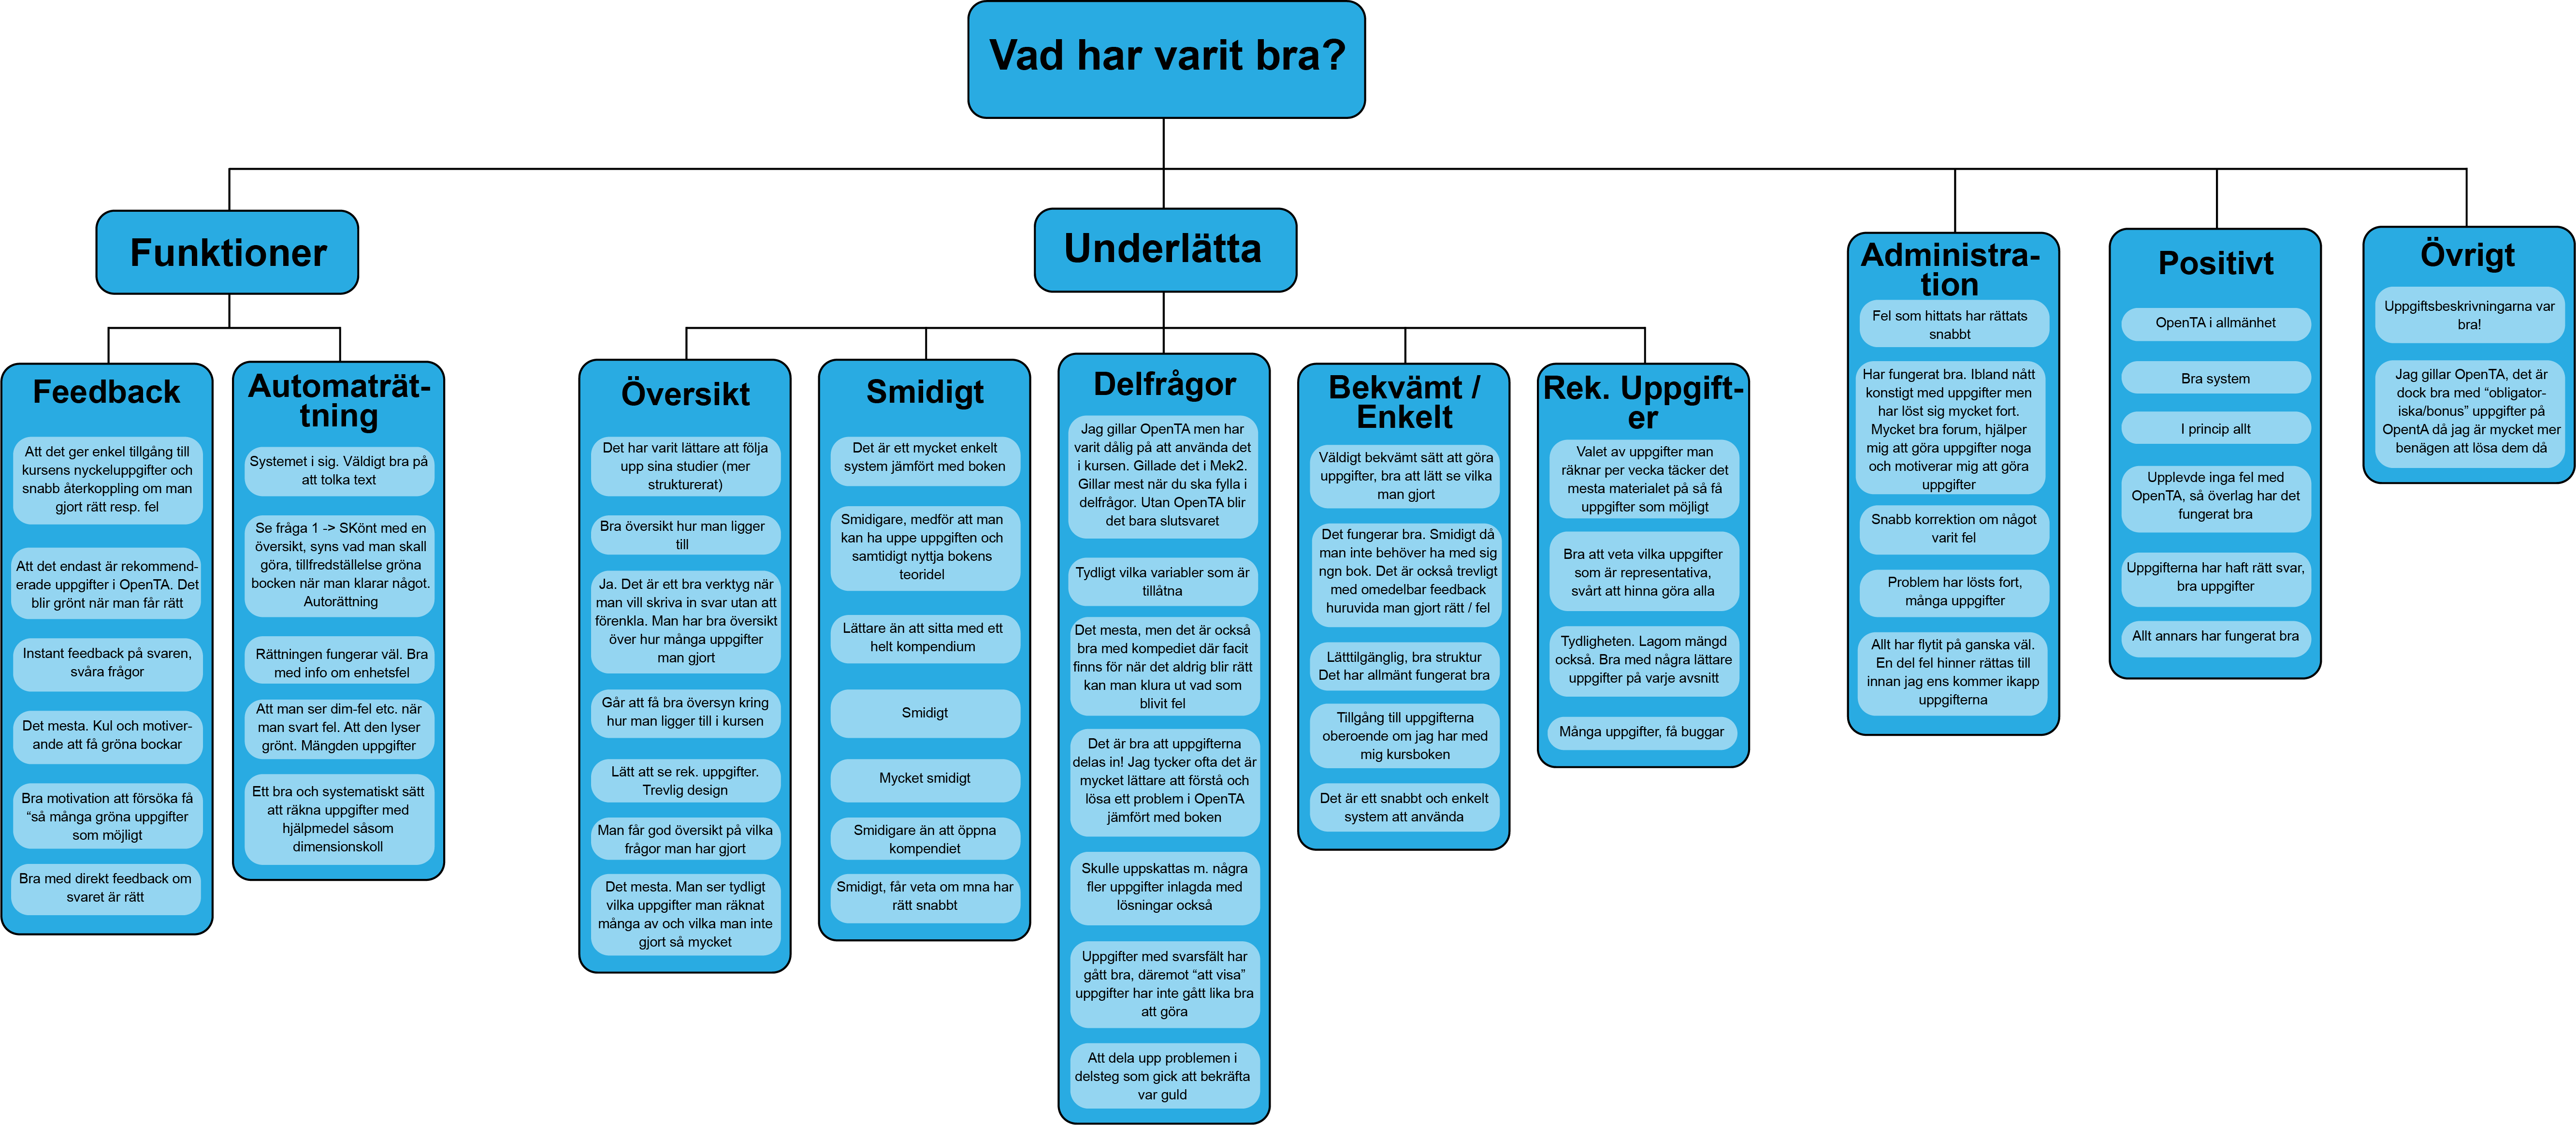
\includegraphics[width=1.0\textwidth]{images/resultpictures/opentakj.png}
    \caption{Resultatet av KJ-analysen från svaren på frågan ''vad har varit bra?''. Specifikt visar rubrikerna för de övergripande sambanden i enkätsvaren, medan de enkilda svaren representerar andelen svar per rubrik. För en version med fullständigt läsbara svar se appendix.}
    \label{fig:raket1}
\end{figure}
\end{center}

Utifrån benchmarkingen noterade vi en trend i att vara tydlig med feedback till användaren visuellt i form av gröna bockar och så kallade progression bars. Men även att hålla gränssnittet avskalat och inte dölja några element. 

\subsection{YATA}
Med förarbetet som grund utvecklade vi applikationen \emph{YetAnotherTA}, eller kort YATA. En demoversion av webbsidan är tillgänglig på https://demo.yata.anton.pizza, där användarnamnet ''demo'' kan användas för inloggning. Nedan presenterar vi webbsidans design och funktionalitet. Vi inleder med ett exempel på en design i Figma och hur samma vy implementerats på webbsidan. Därefter visar vi den övergripande strukturen på sidan och beskriver mer ingående struktur och designval följt av hur dessa har implementerats.   

\begin{center}
\begin{figure}[H]
    \centering
    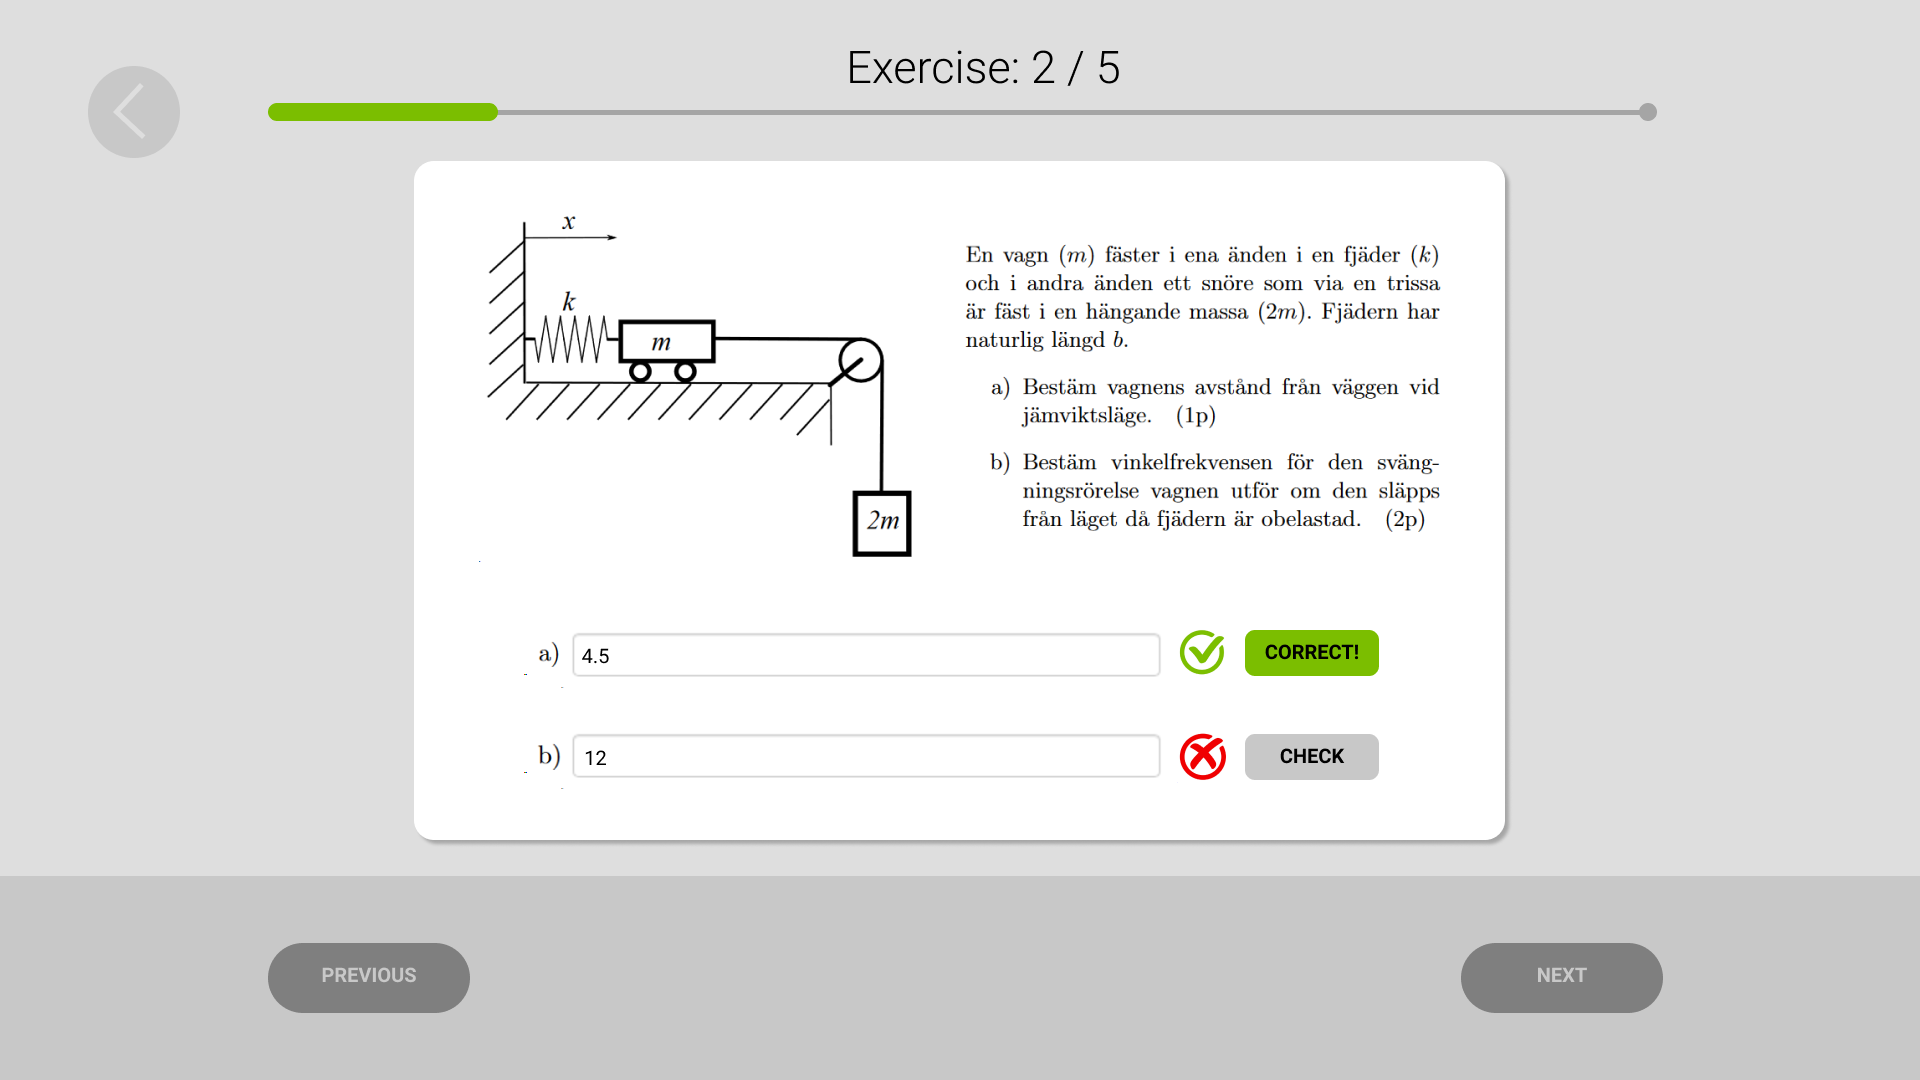
\includegraphics[width=1.0\textwidth]{images/resultpictures/figma_exerciseview.png}
    \caption{Frågevyn som designad i Figma. Överst ges vilken uppgift i kapitlet användaren befinner sig på samt en progression bar som förmedlar hur stor andel av kapitlets uppgifter som är lösta. Därunder lyfts uppgiftstexten och bild fram på en vit bakgrund för att framhålla fokus. I övrigt är andra element mer avskalade för att undvika plottrighet och distraktion.}
    \label{fig:raket2}
\end{figure}
\end{center}

\begin{center}
\begin{figure}[H]
    \centering
    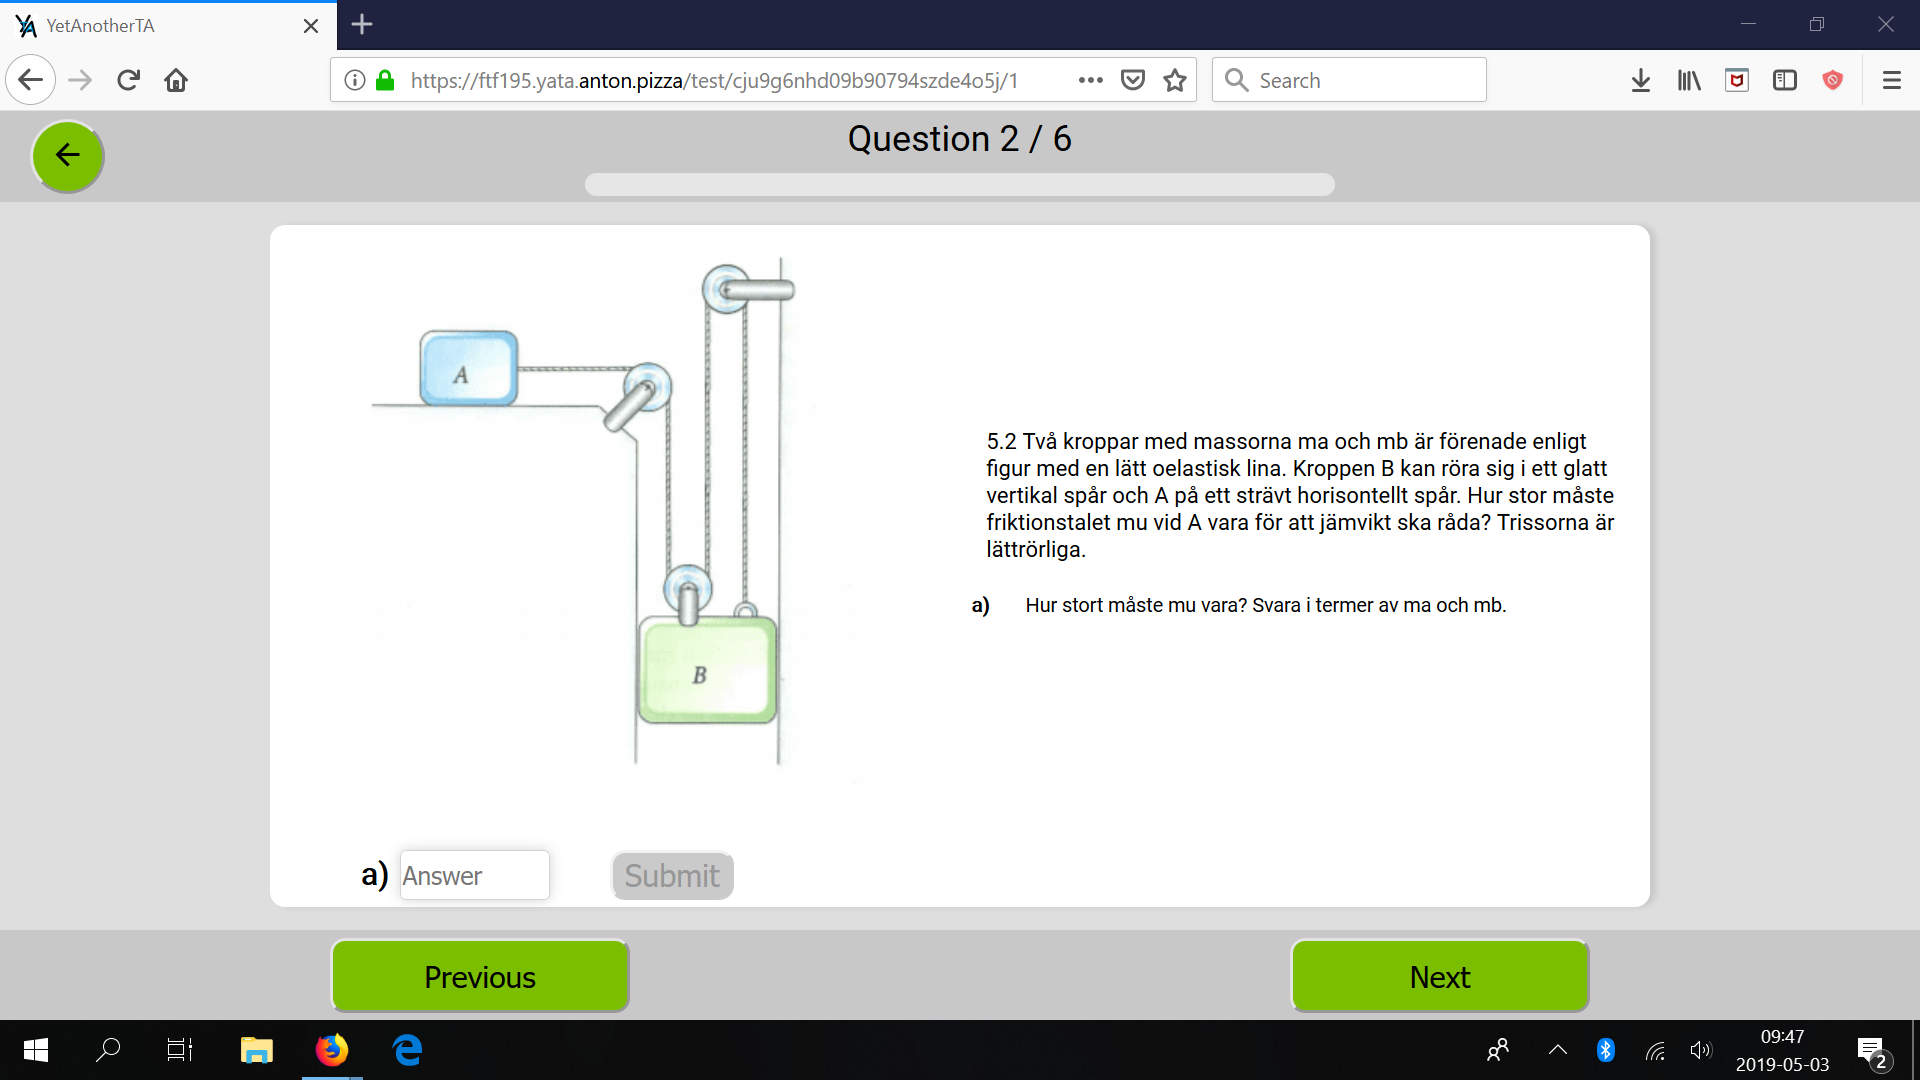
\includegraphics[width=1.0\textwidth]{images/resultpictures/fragevy.png}
    \caption{Implementationen av designen på hemsidan som visad i en webbläsare. Vissa kompromisser har gjorts i implementationen på grund av tidskravet.}
    \label{fig:raket3}
\end{figure}
\end{center}


\begin{center}
\begin{figure}[H]
    \centering
    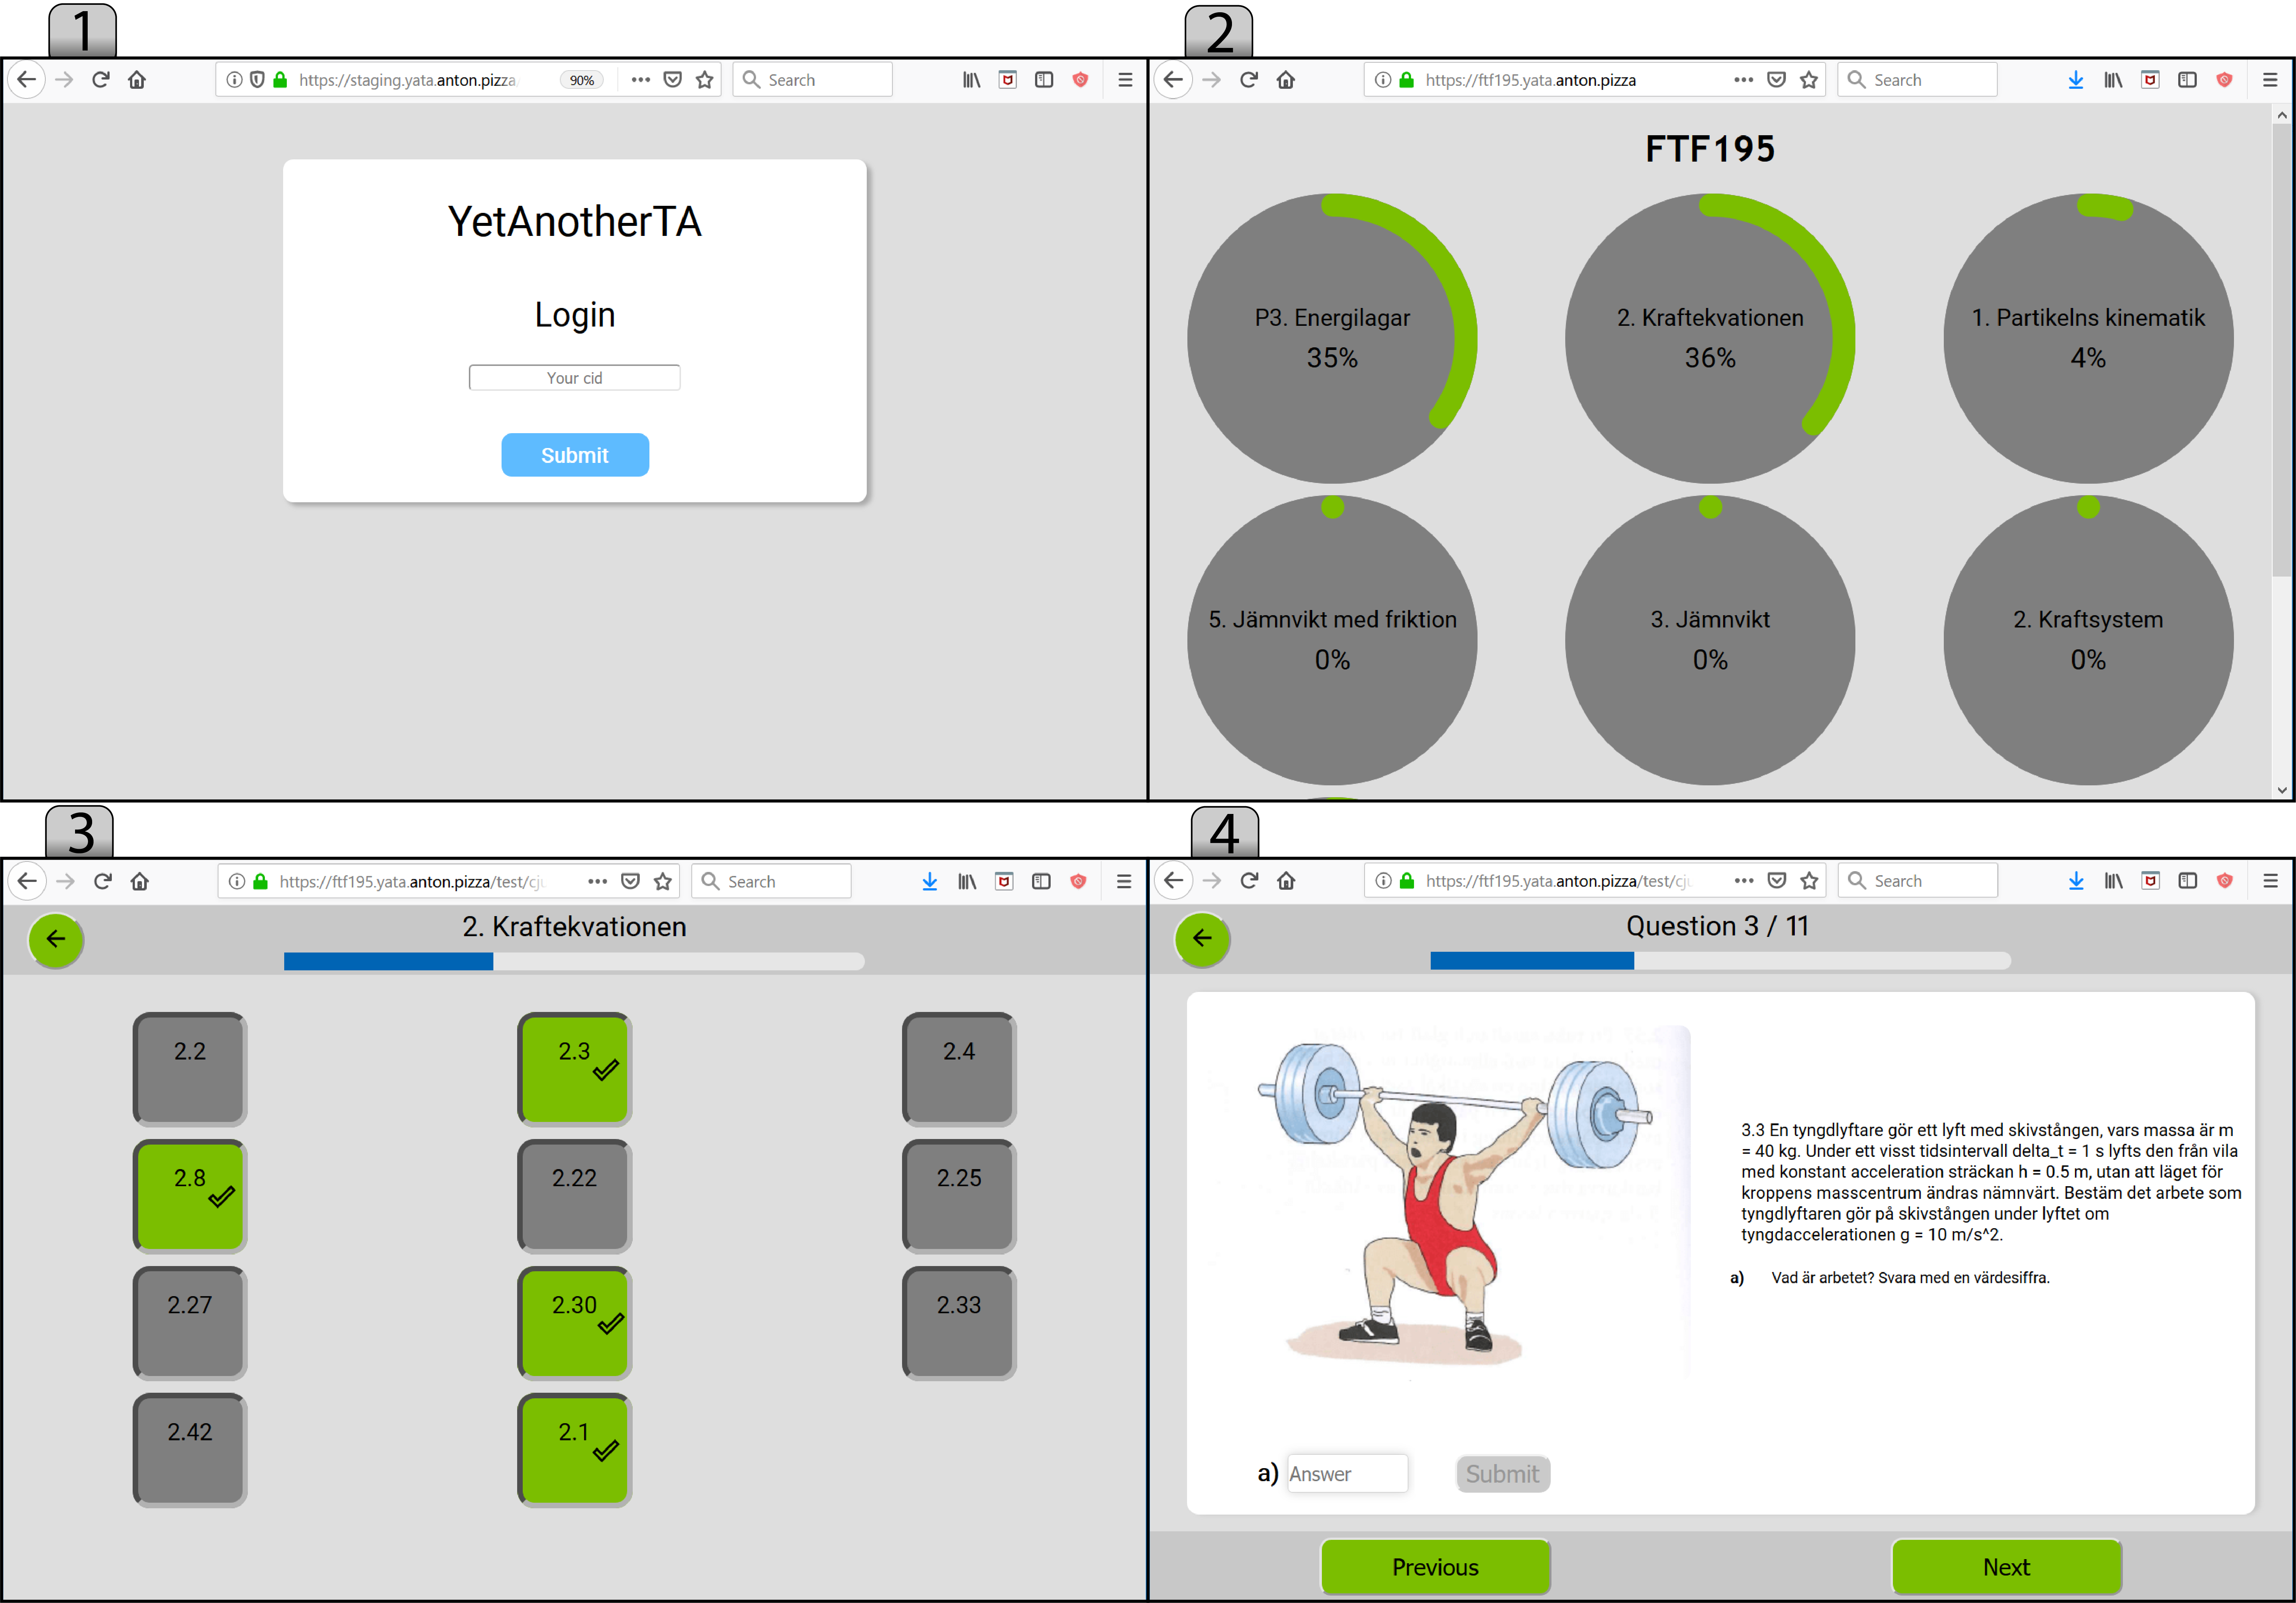
\includegraphics[width=1.0\textwidth]{images/resultpictures/4pics1website.png}
    \caption{De fyra olika vyerna i den grundläggande MVP:n. 1.Login-skärmen, 2. Kapitelvyn, 3. Överisktsvyn och 4. Frågevyn. }
    \label{fig:raket4}
\end{figure}
\end{center}


Eftersom studenterna uppskattade översikt och struktur är detta något som har prioriterats i designen. Efter att ha loggat in ska användaren, i kapitelvyn, snabbt kunna få en överskådlig bild av hur denne ligger till i kursen. Detta genom att användaren ser de olika kapitlen samt hur stor del av uppgifterna i ett kapitel som är lösta, vilket representeras av en procentsats samt ett progressionsfält. För varje kapitel finns en översiktsvy över de olika uppgifterna i kapitlet. Där syns hur många uppgifter kapitlet innehåller samt vilka som är lösta respektive olösta. Överst i denna skärm finns också ett progressionsfält som motsvarar antalet lösta uppgifter i kapitlet. I frågevyn kan sedan användaren effektivt navigera mellan de olika uppgifterna i kapitlet genom knapparna Next och Previous. Användaren kan återgå till översiktsvyn från frågevyn genom tillbakapilen i övre vänstra hörnet. På samma sätt kan användaren komma från översiktsvyn till kapitelvyn. 




%% Teknik, förklara hur klasser och requests representeras bildligt i figurerna ovan.
\subsection{Applikationsflöde grundläggande MVP}
I följande stycken presenteras hur en användare typiskt interagerar med YATA, och hur detta motsvaras i form av data, klassanrop och kommunikation med databasen.

Användaren uppmanas till att mata in sitt CID i login-skärmen, som sedan används i en nätverksförfrågan till databasen. Om användaren inte finns registrerad på kursen fås ett felmeddelande tillbaka. Annars omdirigeras användaren till kapitelvyn för tillgängliga frågesamlingar. I detta stadie kan användaren välja bland de samlingar av uppgifter som presenteras, exempelvis som kapitel ur en lärobok, veckans rekommenderade uppgifter, eller en gammal tentamen. 

När användaren klickar på vald samling uppgifter, kommer ID:t för samlingen att användas med React Router, för att dirigera användaren till övesiktsvyn. Översiktsvyn visar samtliga frågor, och användaren kan även se vilka frågor som är besvarade. Klassen som vyn representerar, baseras mer eller mindre på samma sätt som föregående vy. En query skickas till Apollo-klienten, där frågorna för valt test återfås som en lista. Dessa målas då ut som fyrkanter, och är gröna ifall de har besvarats. Från föregående steg är alla frågor redan sparade i cache-minnet, eftersom listan av frågor innehåller all nödvändig information. Således innebär det att användaren kommer nå vyn för en specifik fråga direkt, utan att behöva vänta på en eventuell query. Klassen som hanterar frågevyn är uppdelad i tre delar: Header, Form och Footer. 

I Form presenteras frågan, med eventuell bild och svarsfält. Form är dynamiskt programmerad, för att alltid anpassa innehållet till skärmens storlek. I footer finns knappar för navigering mellan frågorna. Som tidigare nämnt, är alla frågor sparade i cache-minnet, vilket innebär att navigationen upplevs momentan. När användaren matar in ett svar i någon av fälten anropas funktionen sendAnswer. Metoden begär vid anrop en mutation från Apollo-klienten, som först lägger till svaret i databasen, för att sedan returnera om svaret var rätt eller fel. Responsen kommer i klassen som sedan motsvaras av en grön bock eller ett rött kryss, som användaren ser. 

\subsection{Vidare utvärderingar}


Under utvärderingen från första kursen i läsperiod 3 mottogs feedback för att förbättra användningen. Till exempel att inmatningsfältet ska bli större eller att svar ska stå kvar i inmatningsfältet då användaren lämnar uppgiften och kommer tillbaka senare. För fulla listan av förbättringspunkter, se appendix. 

Slutsatsen av brukarstudien av Piazza var att forumet inte användes i någon större utsträckning av majoriteten av studenterna. Vi identifierade flera anledningar till detta, till exempel att många är rädda för att ställa en fråga i forumet, men också på grund av att svarstiden är långsam. Vi identifierade en form av hierarki efter hur studenter söker efter hjälp när de kört fast. Trenden är studenterna börjar med att googla på problemet. Om hjälp inte fås där är ett vanligt nästa steg att studenten går till sociala medier, exempelvis en gruppchatt på Facebook med sina närmsta vänner. Hjälper heller inte det är det nästa steget studenten frågar en annan kursare nära till hands. Till sist använda PIazza om frågan fortfarande är oläst. En tolkning av detta är att studenterna värdesätter svarstiden högre än kvalitén på svaren.

\begin{center}
\begin{figure}[hbtp]
    \centering
    \hspace{-20px}
    \resizebox {1\textwidth} {!} {
        \definecolor{klight_green_400}{RGB}{156, 204, 101}



\begin{tikzpicture}[x=1.5cm, y=1.5cm, ->,>=stealth',auto, thick, line width=0.5mm]
\tikzset{%
  project part/.style={
    rectangle,
    draw,
    fill=klight_green_400,
    thick,
    minimum width=3.2cm,
    minimum height=1.2cm
  },
  main line/.style={
    draw,
    line width=0.25mm,
    opacity=1,
    minimum size=1cm
  },
}
% Base project nodes
\node [project part/.try] (control) at (0,0) {$\textbf{Google}$};
\node [project part/.try] (predict) at (3,0) {$\textbf{Gruppchatt}$};
\node [project part/.try] (form) at (6,0) {$\textbf{Kursare}$};
\node [project part/.try] (interview) at (9,0) {$\textbf{Piazza}$};


% Connect them 
\path[main line/.style={font=\sffamily\small}]
    (control) edge[right] node [left] {} (predict)
    (predict) edge[right] node [left] {} (form)
    (form) edge[right] node [left] {} (interview);
\end{tikzpicture}

    }
    \caption{En representation av hierarkin i vilken många studenter tycks söka efter hjälp. För en bild av den fullständiga KJ-analysen där denna hierarki identifierades, se appendix \ref{app:KJ-analys}. }
    \label{fig:raket5}
\end{figure}
\end{center}

\subsection{MVP A}

Utifrån den insamlade informationen föreslogs ett antal koncept som skulle kunna uppfylla de behov vi såg, se appendix för listan av koncept. Det koncept vi slutligen bestämde oss för, vad vi kallat MVP A, är en typ av tipsfunktion. Detta med tanke på att studenterna efterfrågade tips i första utvärderingen av OpenTA. Det kan också vara ett mycket snabbt sätt att få hjälp om personen har kört fast, vilket vi upptäckte var viktigt i brukarstudien av Piazza. Tanken är att tipsen ska genereras av användarna själva. Den som löst en uppgift får möjligheten att skriva in ett tips som kan underlätta lösningen. Om någon då har kört fast på samma uppgift kan den personen efterfråga ett tips. En uppgift ska kunna ha flera tips vilket gör att en typ av rangordning bör finnas. Vår tanke är att användarna ska kunna ge ett tips ''tumme upp'' eller ''tumme ner''. Det högst rankade tipset ska då visas först för studenten vid efterfrågan. Tipsfunktionen kan även ge extra datapunkter för djupinlärningen, såsom hur många som efterfrågar tips, hur många som skriver tips eller ger ''tumme upp'' osv. 

I nästkommande stycke beskrivs utvecklingen av MVP A på en mer teknisk nivå.

\begin{center}
\begin{figure}[H]
    \centering
    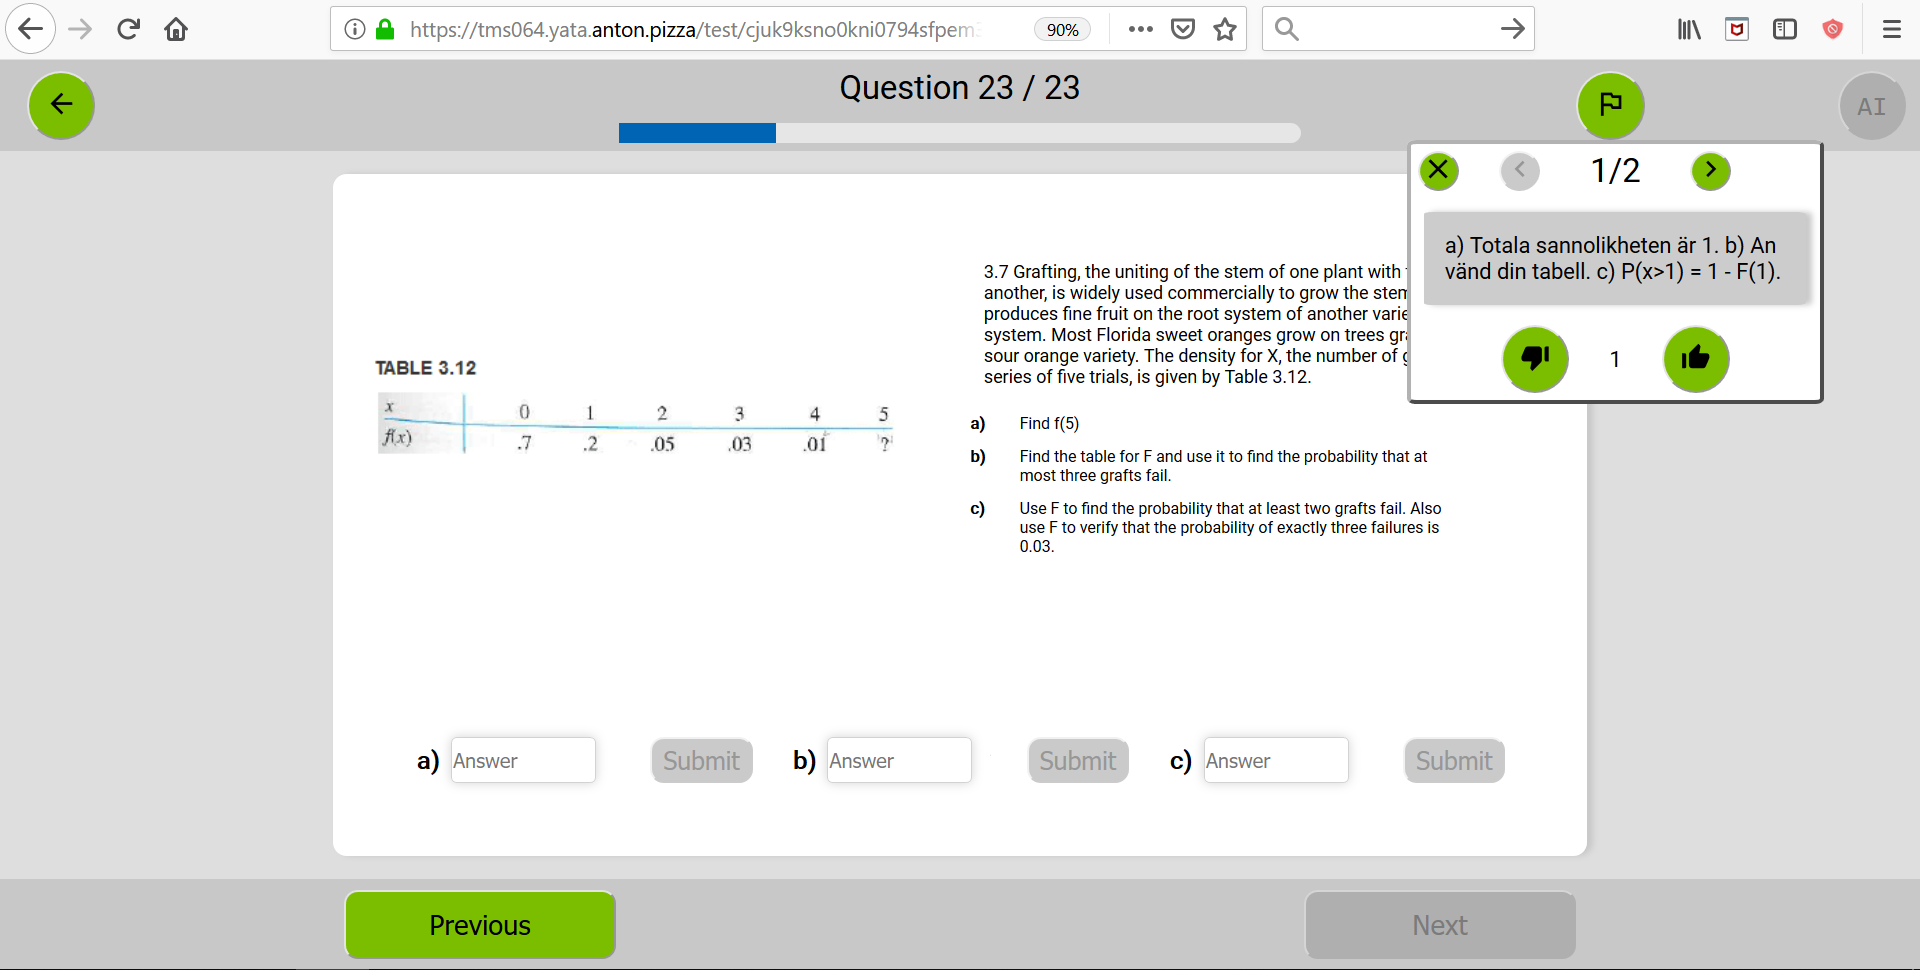
\includegraphics[width=1.0\textwidth]{images/resultpictures/tipsfunktion3.png}
    \caption{Tipsfunktionen i frågevyn. Genom att trycka på flaggan kan studenten få ett tips på hur uppgiften kan lösas.}
    \label{fig:raket6}
\end{figure}
\end{center}

%%Tekniskt stycke, hur funkar tipsfunktion rent kodmässigt med klasser och requests
\subsection{Implementation av MVP A}
I följande stycke beskrivs den tekniska implementationen av MVP A. Här redogörs exempelvis för beslut angående prestanda, säkerhet och koddesign.

Tips-funktionen förändrar inget av den tidigare beskrivna implementationen, utan motsvarar endast tillagd funktionalitet. När användaren trycker på tips-knappen renderas modal-panelen där tipsen syns, och en query skickas till Apollo-klienten, där svaret innehåller det högst röstade tipset. Användaren kan sedan navigera mellan tipsen, och vid en eventuell rörelse kommer en ny query skickas till Apollo-klienten på samma sätt. Anledningen till att alla tips inte sparas i cache-minnet är av två skäl. 

Först och främst hade det inneburit att en användare med enklare erfarenheter av webbutveckling kan komma åt samtliga tips i nätverksloggen, vilket i sin tur innebär att djupinlärningsalgoritmerna inte med säkerhet kan veta om användaren tagit hjälp av tips. För det andra hade det även försvårat processen att manuellt avgöra hur många tips en användare tagit hjälp av. För enkelhetens skull kan istället anropet till Apollo-klienten för varje tips användas som referens till algoritmen.

En användare kan även rösta på existerande tips, för att förbättra relevansen hos tipsen. De två ''tummarna'' motsvarar då antingen +1 eller -1. När en användare röstar anropas en liknande mutation som vid ovan nämnt bevarande av en fråga. I mutationen skickas antingen +1 eller -1, och responsen innehåller tipset användaren röstat på. Detta för att uppdatera cache-minnet (med enbart den frågan), eftersom då användaren kan se förändringar.

När en användare besvarat samtliga delfrågor för en uppgift, visas en en modal där användaren uppmanas dela sitt mest betydelsefulla tips för frågan. Anledningen bakom att uppmana användaren på ett så avbrytande vis, är för att fånga så många svar som möjligt. Ett problem hade annars kunnat vara att användaren glömmer att lämna ett tips. När användaren slutligen lämnar ett tips anropas en mutation till Apollo-klienten, som tar in svaret, och returnerar resultatet i form av en boolsk variabel.

\begin{center}
\begin{figure}[H]
    \centering
    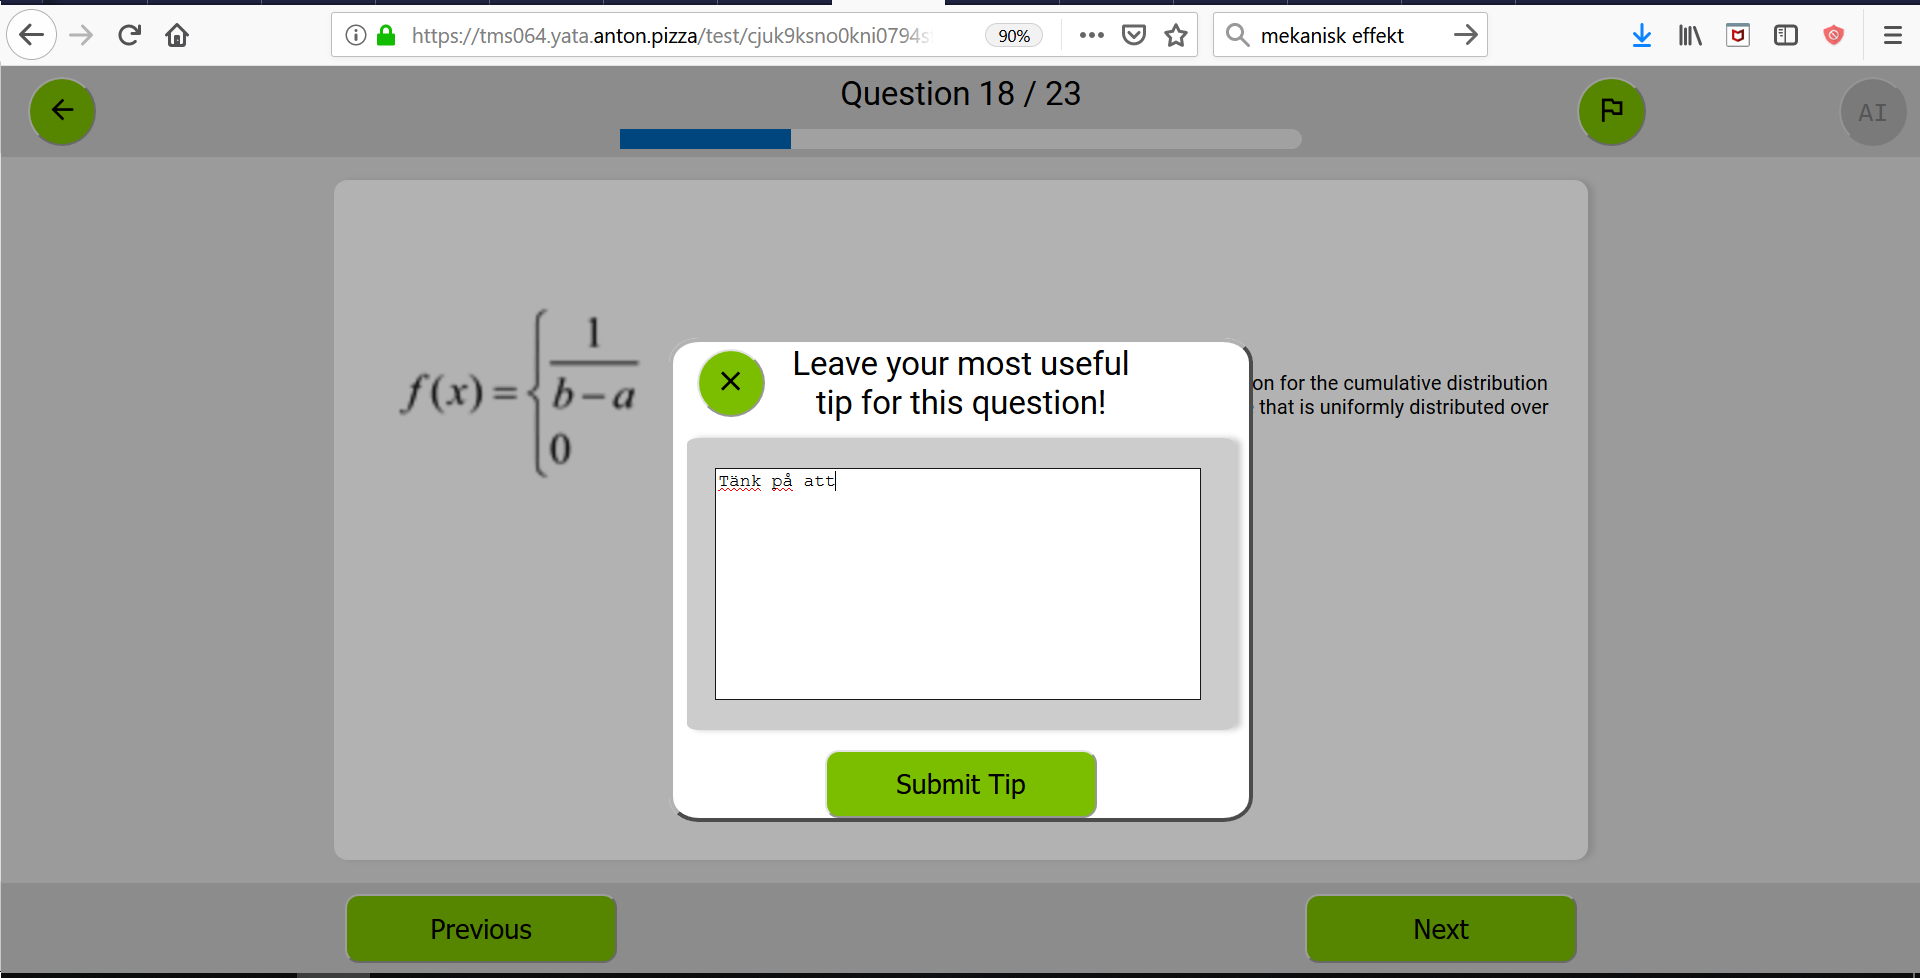
\includegraphics[width=1.0\textwidth]{images/resultpictures/tipsfunktion2.png}
    \caption{När en uppgift är löst får användaren möjlighet att skriva in ett tips för hur uppgiften kan lösas.}
    \label{fig:raket7}
\end{figure}
\end{center}

\section{Diskussion}
\label{sec: webb-D}

De behov och krav som identifierats kan i stora drag delas in i två huvudkategorier: behov och krav kring studier i allmänhet samt specifikt kring webbplattformar. Vad vi identifierat kring studier i allmänhet är att studenterna överlag har en vilja att lösa uppgifterna på egen hand. Ibland kör de emellertid fast i lösningsgången och har då ett behov av hjälp på något sätt. Vår tolkning av hierarkin vi identifierade i brukastudien av Piazza är att många värderar svarstiden högre än kvalitén på svaret när de söker efter hjälp. Att maila föreläsaren eller fråga på Piazza hade förmodligen genererat ett svar av hög kvalité, dock är svarstiden ofta långsam. Ett citat från en av intervjuerna är ''det känns bättre att googla i fem minuter än att vänta i fem minuter'', vilket visar på ett tydligt behov av att få hjälpen direkt. Ytterligare något vi observerade var att studenterna överlag drar sig för att ställa frågor i större öppna forum, men om de gör det är anonymitet ett krav. Det finns en viss rädsla för att fråga om hjälp i mer offentliga sammanhang, även om det är i en digital miljö som ett forum. Studenterna känner sig mer trygga att fråga om hjälp i en mindre gruppchatt med sina nära vänner till exempel. Allra först dock, söker många hjälp via Google. Förmodligen för att det är mest lättillgängligt, men också kanske för att det inte är en social miljö på samma sätt som ett forum eller en gruppchatt. 

Tipsfunktionen är utformad med tanke på dessa aspekter. Den erbjuder ögonblicklig hjälp om det finns skrivna tips samtidigt som det är anonymt att ta hjälp av tipsen. Pedagogiskt kan den också vara bättre för att folk kan få hjälp i sin lösningsgång, utan att först kolla i facit, samt för att den som skriver in ett tips får reflektera över uppgiften i efterhand, vilket kan vara är positivt för inlärningen. Vad vi sett från några tidiga observationer av användningen av tipsfunktionen är att studenter har skrivit in tips och gett ”tumme upp” vilket indikerar att åtminstone vissa av studenterna finner ett värde i tipsfunktionen. Vad vi också sett är att vissa skrivit in det korrekta svaret, dvs facit, i tipsrutan, vilket är ett intressant beteende vars orsak borde undersökas. En rigorös utvärdering av hur tipsfunktionen fungerat och hur studenterna använt den bör göras efter läsperiodens slut. 

Vad gäller behov och krav för webbplattformar uppskattar, som tidigare nämnt, många studenter översikt och struktur. Till exempel, att samla och strukturera upp de rekommenderade uppgifterna på ett ställe samt att det automatiskt hålls koll på vilka uppgifter som  är lösta och inte. Det blir är annars ett extra administrativt moment för studenten. Att webbsidan gör detta innebär att studenterna sparar mer tid, vilket effektiviserar deras studier. När studenterna interagerar med dessa plattformar vill de också ha direkt och tydlig feedback i sin interaktion. I många andra inlärningsprogram till exempel gavs positiv feedback även vid allra minsta framsteg, som en motivationsfaktor för studenten. Ytterligare ett krav på direkt och tydlig feedback har studenterna vad gäller svarshanteringen. I dagsläget har de svårt att skilja på om svaret är inmatat på fel form, om det är syntaxfel, eller om svaret helt enkelt är fel. Detta är något som studenterna vill ha bättre återkoppling på. I vidare utveckling är en svarshantering med mer direkt feedback ett utvecklingsområde. 


%%Något som studenterna efterfrågade både i den första informationsinsamlingen samt de vidare utvärderingarna var facit för uppgiften. På dessa hemsidor finns inte facit tillgängligt på samma sätt som i en lärobok till exempel, där svaren oftast finns längst bak. Att inte ha facit kan vara positivt ur ett inlärningsperspektiv eftersom man då inte ”fuskar” i lösningsgången. Många vill dock kunna kontrollera sina svar mot facit, eller om man kört fast ''back-tracka'' en lösning från facit. 